
\documentclass{article}
\usepackage{graphicx}
\usepackage{apacite}
\usepackage{natbib}

\begin{document}

\title{One-Dimensional Approximation of a Multi-Dimensional Neuronal System}
\author{Joaquin Rapela\thanks{rapela@ucsd.edu}}

\maketitle

\section{Theory}

The dynamics of a \textbf{multi-dimensional} dynamical system near a
saddle-node bifurcation can be reduced to that of the \textbf{one-dimensional}
topological normal form~\citep[][p.163]{izhikevich07}:

\begin{eqnarray}
\dot{V}=c(b-b_{sn})+a(V-V_{sn})^2
\label{eq:qifModel}
\end{eqnarray}

\noindent where

\begin{eqnarray}
a&=&\frac{1}{2}\frac{\partial^2\mathbf{I}(V, b_{sn})}{\partial V^2}\Bigg|_{V=V_{sn}}
\label{eq:a}\\
c&=&\frac{\partial\mathbf{I}(V_{sn}, b)}{\partial b}\Bigg|_{b=b_{sn}}
\label{eq:c}
\end{eqnarray}

\noindent $b$ represents the bifurcation parameter, and ($b_{sn}, V_{sn}$) is
the bifurcation point.

\vspace{0.1in}

\noindent \textbf{Note}: by \emph{near a saddle-node bifurcation} we mean
that the trajectory of the neuronal system should pass close to a saddle-node
bifurcation point.

\section{Example INap+IK model}

An INap+IK model with high-threshold parameters undergoes a saddle-node
bifurcation at $V_{sn}=-60.9325$ and $n_{sn}=0.0007$, with
$I_{sn}=4.51$~\citep[][Example: The INap+IK-model on page 163]{izhikevich07}.
With these parameters we obtain $a=0.1887$ and $c=1$ from Eqs. \ref{eq:a}
and~\ref{eq:c}. Thus, the equivalent one-dimensional model takes the form:

\begin{eqnarray}
\dot{V}=(I-4.51)+0.1887(V+60.9325)^2
\end{eqnarray}

\noindent which can be solved analytically. For $I>I_{sn}$ the solution is:

\begin{eqnarray}
V(t)=V_{sn}+\sqrt{\frac{c}{a}(I-I_{sn})}\tan(a\,c\,(I-I_{sn})\,t+c_0)
\end{eqnarray}

If we reset the voltage to $V(t+\Delta t)=V_{reset}$ when $V(t)>V_{thr}$, we
obtain the Quadratic Integrate and Fire (QIF) model~\citep[][p.
80]{izhikevich07}.

For different values of the input current,
Figures~\ref{fig:INap+IKAndQIF_tauV1.00I4.58}-\ref{fig:INap+IKAndQIF_tauV1.00I9.00}
plot the phase space of the INap+IK model and its voltage traces along with
the voltage traces of the QIF model~\footnote{We have added a constant delay
of 5.1~ms at times when the voltage reaches threshold (i.e., $V(t)=V_{thr}$)
to account for the approximately constant spike generation time in the INap+IK
model.}.

\begin{figure}
\begin{center}
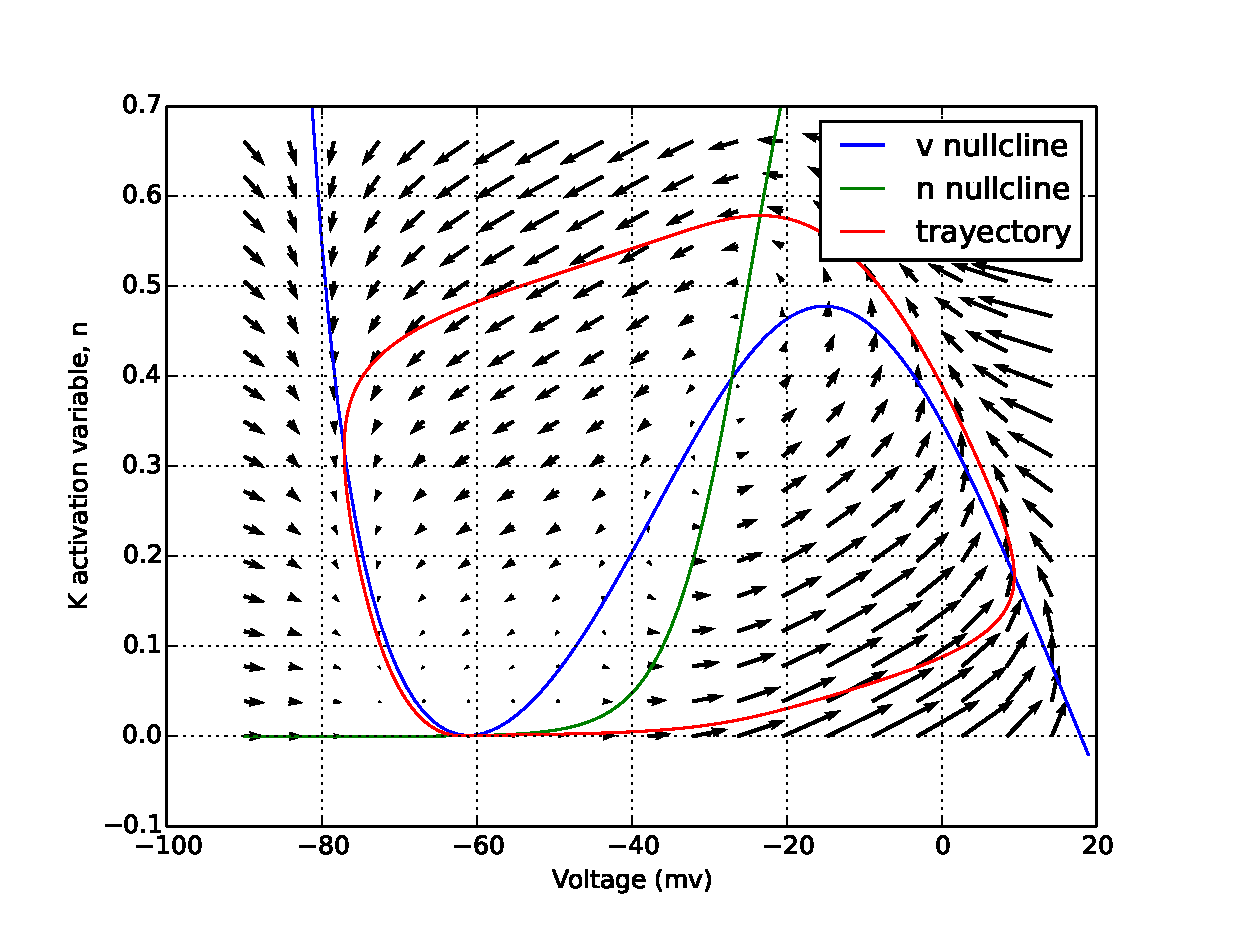
\includegraphics[width=4.5in]{../../figures/fig6-07PhaseSpaceTauV1.00I4.58.eps}
\includegraphics[width=4.5in]{../../figures/qIFAndINapIKSolutionsTauV1.00I4.58.eps}

\caption{Top: phase space of the INap+IK model with high-threshold parameters.
Bottom: voltage trace of the INap+IK model (green trace), and its
approximation by a QIF model (blue trace). Input current 4.58 mA.}

\label{fig:INap+IKAndQIF_tauV1.00I4.58}
\end{center}
\end{figure}

\begin{figure}
\begin{center}
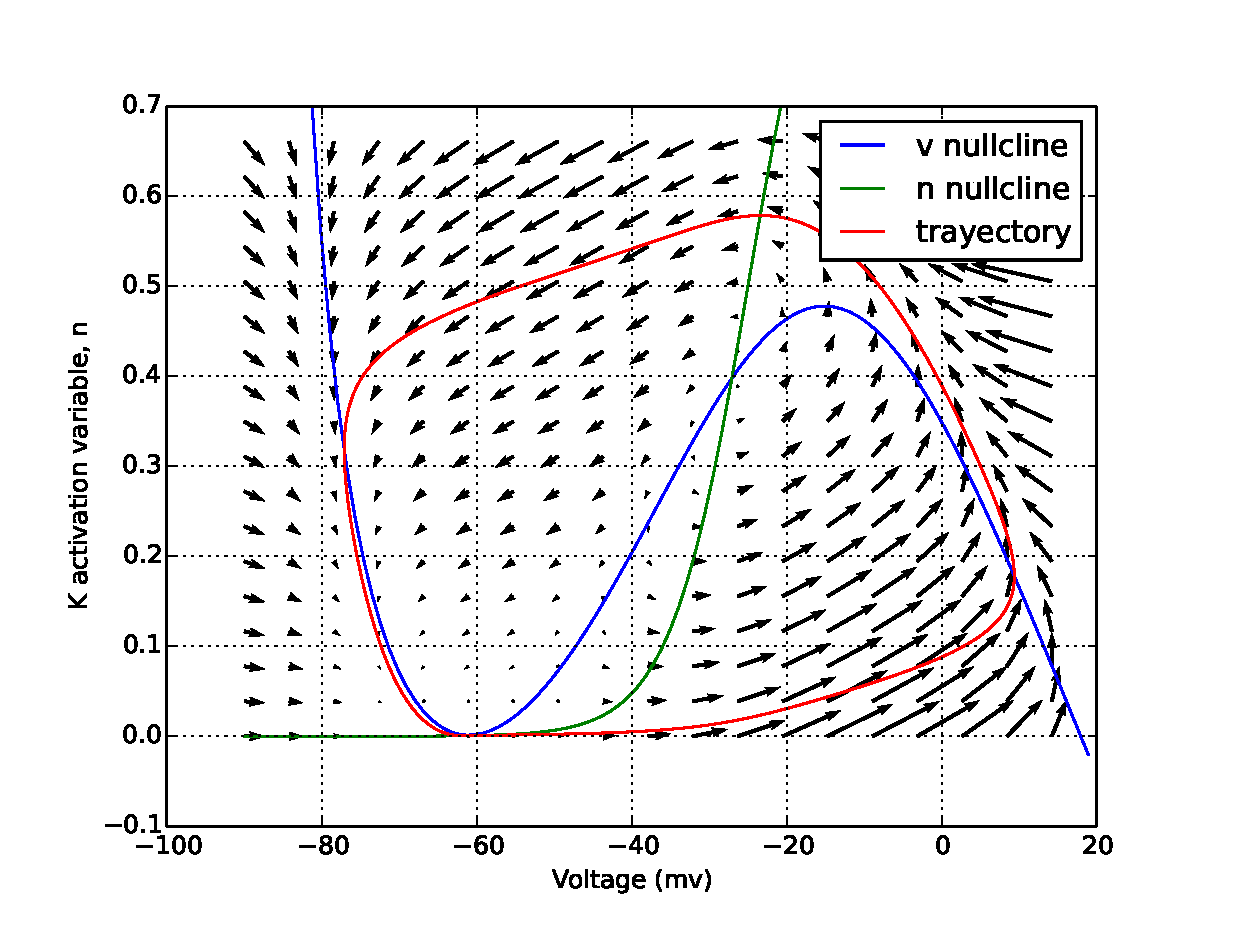
\includegraphics[width=4.5in]{../../figures/fig6-07PhaseSpaceTauV1.00I4.65.eps}
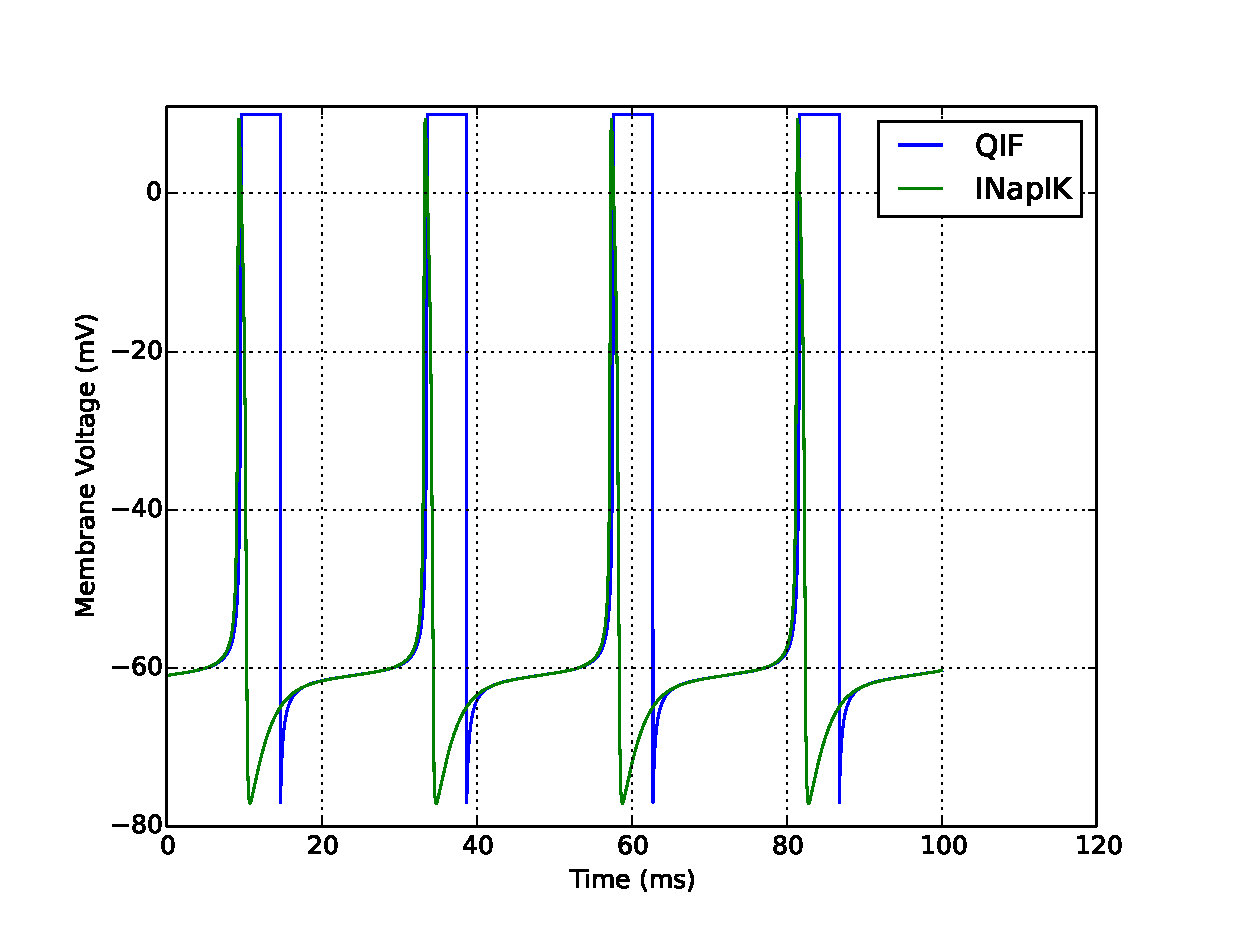
\includegraphics[width=4.5in]{../../figures/qIFAndINapIKSolutionsTauV1.00I4.65.eps}

\caption{Top: phase space of the INap+IK model with high-threshold parameters.
Bottom: voltage trace of the INap+IK model (green trace), and its
approximation by a QIF model (blue trace). Input current 4.65 mA.}

\label{fig:INap+IKAndQIF_tauV1.00I4.65}
\end{center}
\end{figure}

\begin{figure}
\begin{center}
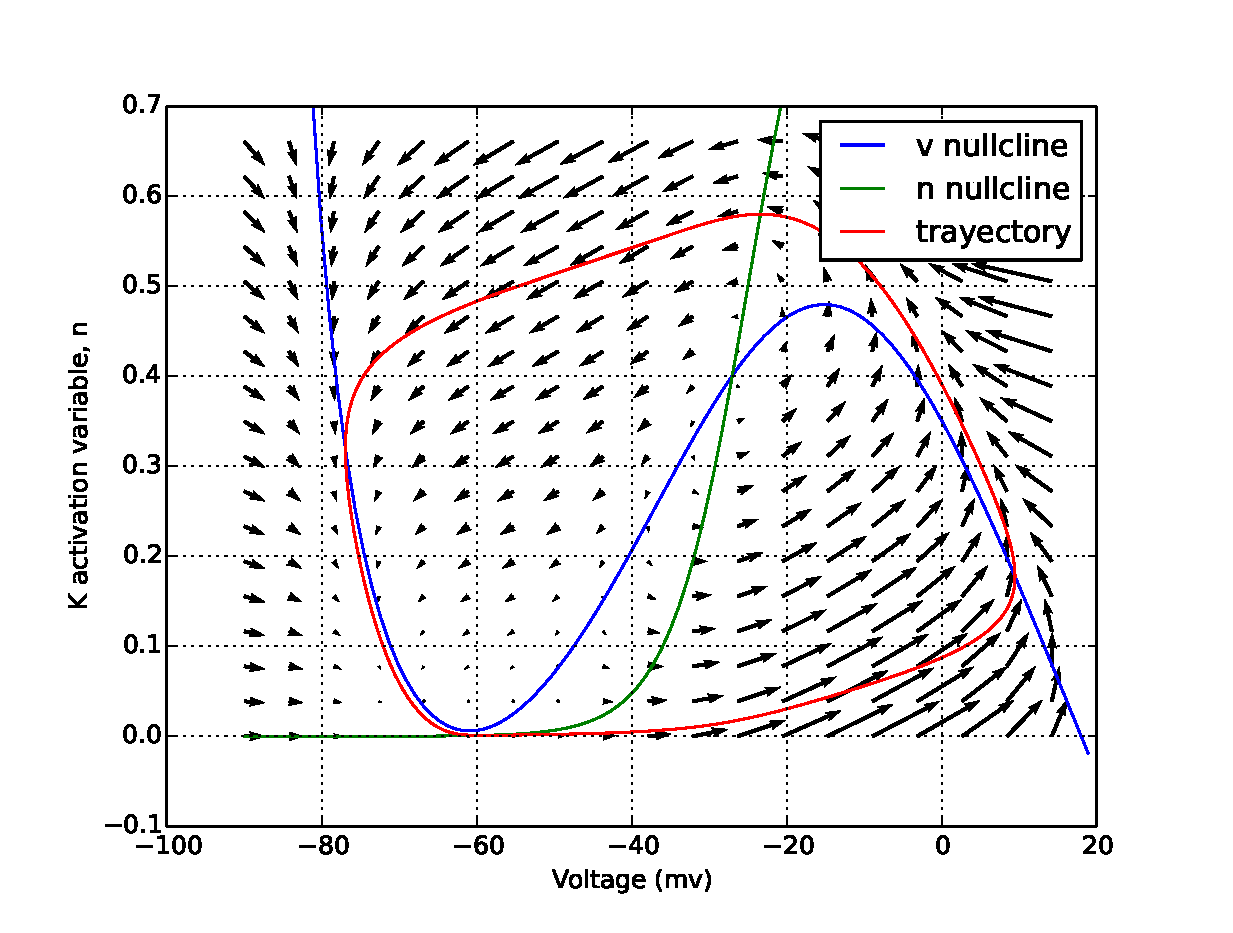
\includegraphics[width=4.5in]{../../figures/fig6-07PhaseSpaceTauV1.00I6.00.eps}
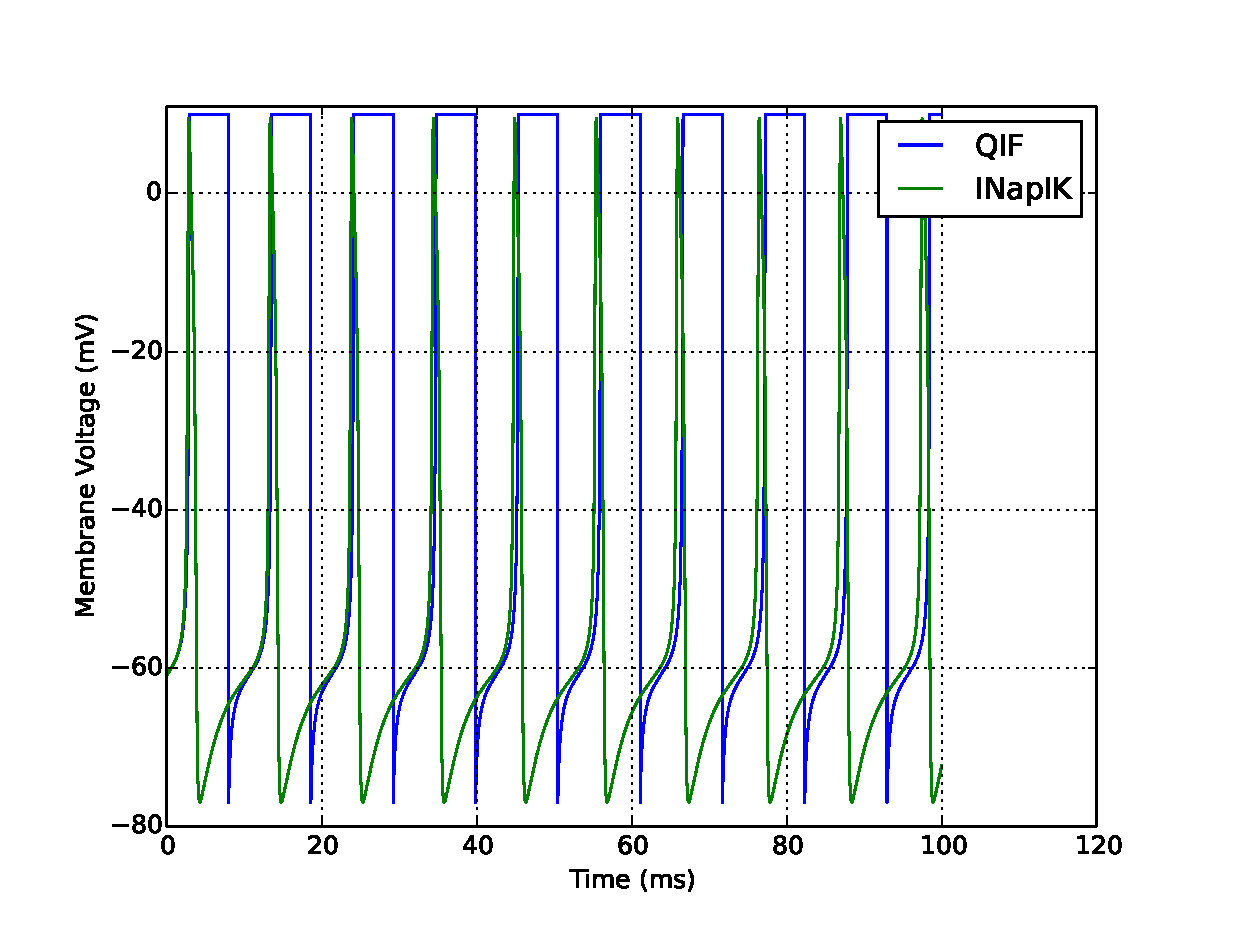
\includegraphics[width=4.5in]{../../figures/qIFAndINapIKSolutionsTauV1.00I6.00.eps}

\caption{Top: phase space of the INap+IK model with high-threshold parameters.
Bottom: voltage trace of the INap+IK model (green trace), and its
approximation by a QIF model (blue trace). Input current 6.00 mA.}

\label{fig:INap+IKAndQIF_tauV1.00I6.00}
\end{center}
\end{figure}

\begin{figure}
\begin{center}
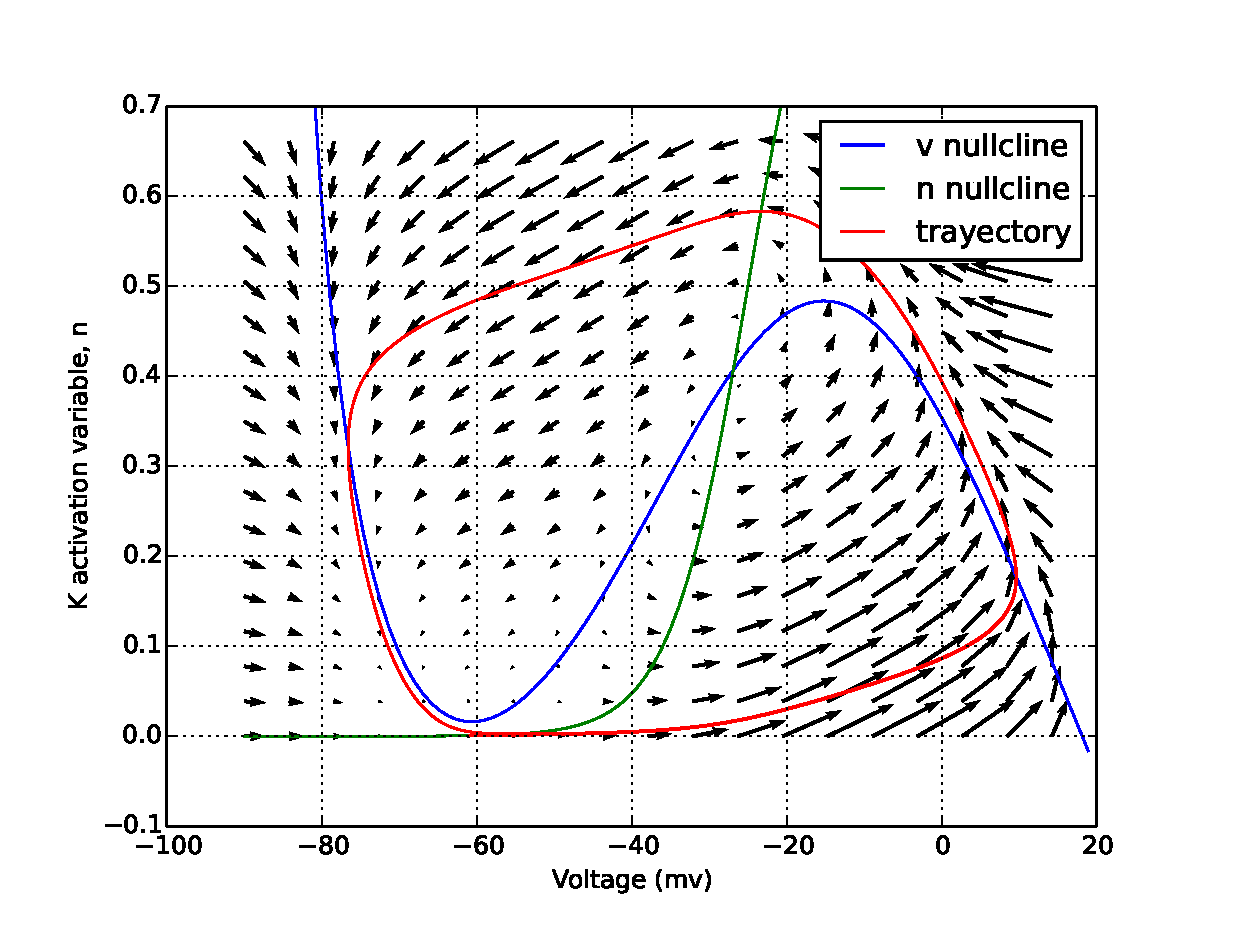
\includegraphics[width=4.5in]{../../figures/fig6-07PhaseSpaceTauV1.00I9.00.eps}
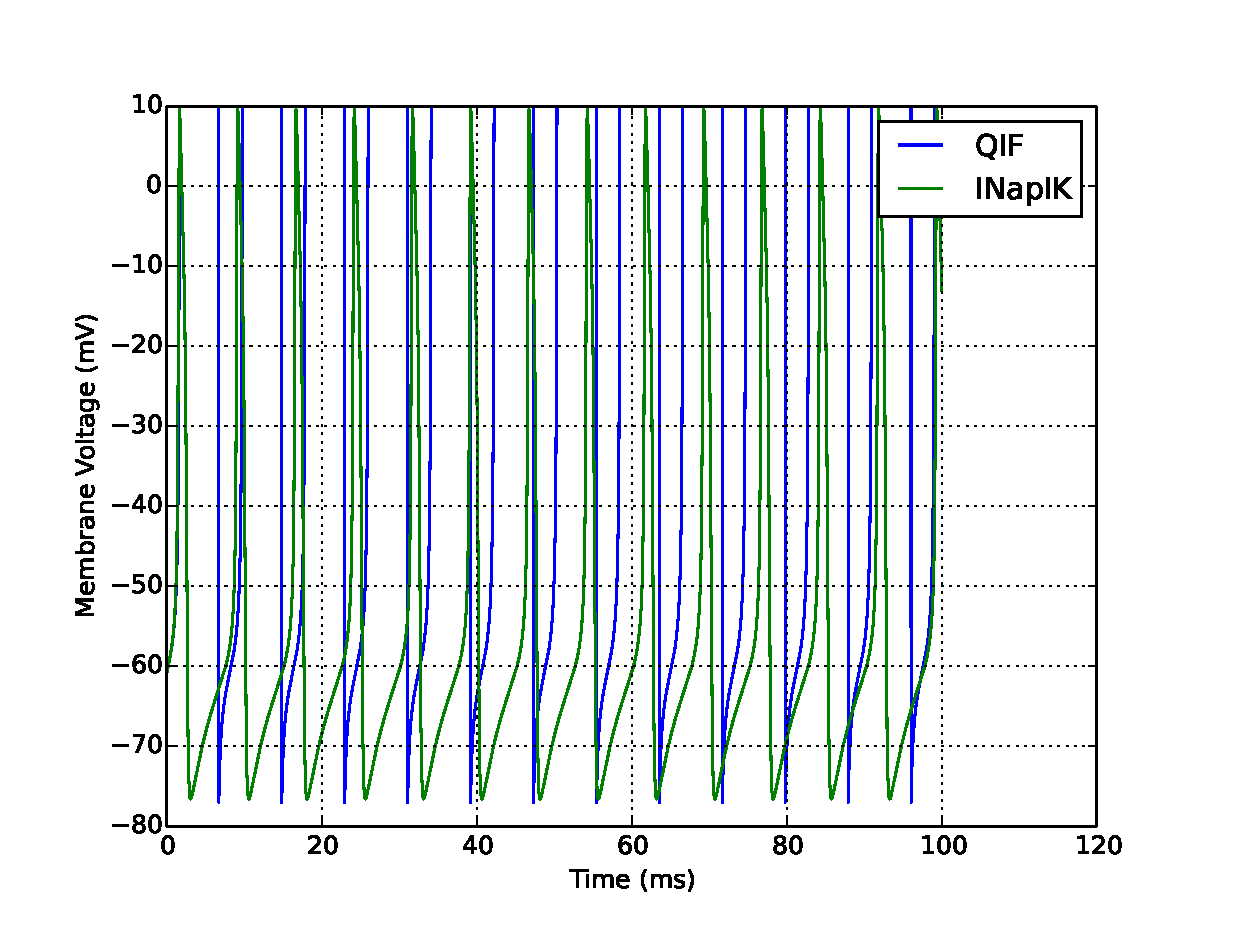
\includegraphics[width=4.5in]{../../figures/qIFAndINapIKSolutionsTauV1.00I9.00.eps}

\caption{Top: phase space of the INap+IK model with high-threshold parameters.
Bottom: voltage trace of the INap+IK model (green trace), and its
approximation by a QIF model (blue trace). Input current 9.00 mA.}

\label{fig:INap+IKAndQIF_tauV1.00I9.00}
\end{center}
\end{figure}

The phase spaces in the top panels of
Figures~\ref{fig:INap+IKAndQIF_tauV1.00I4.58}-\ref{fig:INap+IKAndQIF_tauV1.00I9.00}
show that for the chosen parameters and input current values the INap+IK model
is close to the saddle-node bifurcation. Therefore, the QIF should be a good
approximation, as demonstrated by the voltage traces in the bottom panels of
Figures~\ref{fig:INap+IKAndQIF_tauV1.00I4.58}-\ref{fig:INap+IKAndQIF_tauV1.00I9.00}.
However, if we change the time constant of the $n$ gating variable of the
INap+IK model from 1.0 to 0.152 and use an input current $I=5.0$, the
trajectory INap+IK model moves away from the saddle-node bifurcation point and
its approximation by the QIF model becomes poor, as illustrated in
Figure~\ref{fig:INap+IKAndQIF_tauV0.15I5.00}.

\begin{figure}
\begin{center}
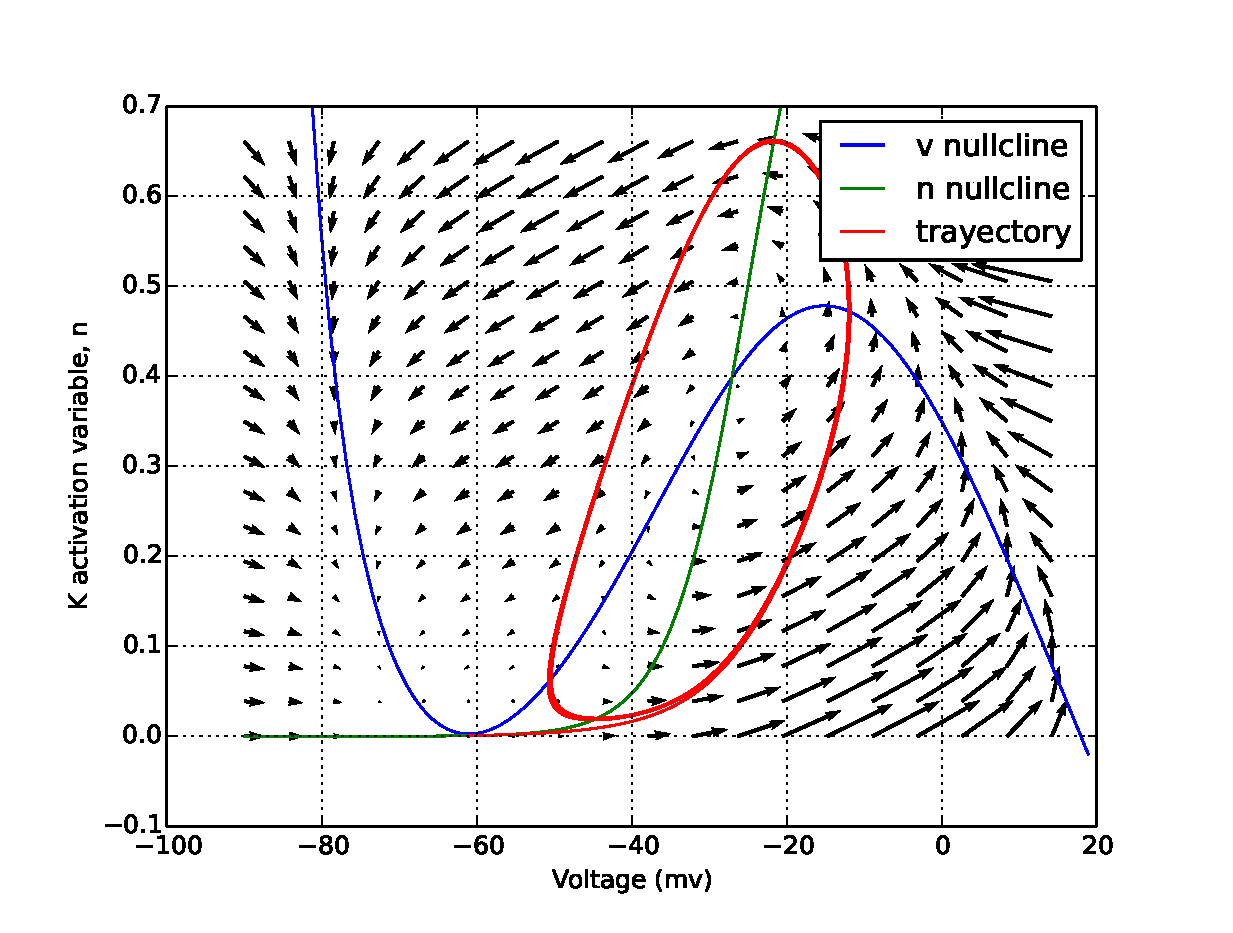
\includegraphics[width=4.5in]{../../figures/fig6-07PhaseSpaceTauV0.15I5.00.eps}
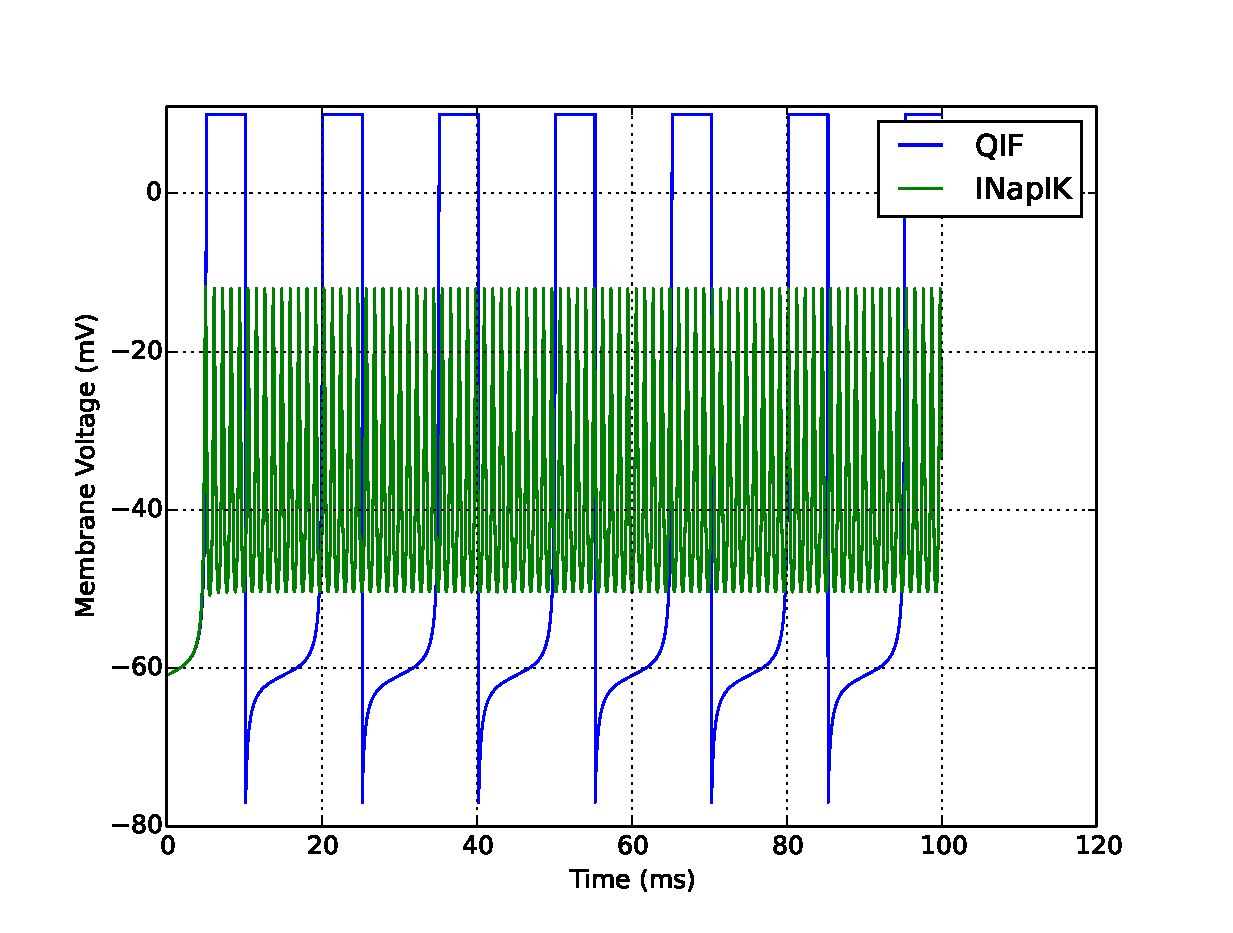
\includegraphics[width=4.5in]{../../figures/qIFAndINapIKSolutionsTauV0.15I5.00.eps}

\caption{Top: phase space of the INap+IK model with high-threshold parameters
and fast K current (i.e.; $\tau(V)=0.152$)..
Bottom: voltage trace of the INap+IK model (green trace), and its
approximation by a QIF model (blue trace). Input current 5.00 mA.}

\label{fig:INap+IKAndQIF_tauV0.15I5.00}
\end{center}
\end{figure}

\bibliographystyle{apacite}
\bibliography{dynamicalSystems}

\end{document}
